\documentclass{scrartcl}

%\pagestyle{empty}		% keine Kopf und Fu�zeile (k. Seitenzahl)
%\pagestyle{headings}	% lebender Kolumnentitel  

\usepackage[ngerman]{babel}
\usepackage[T1]{fontenc}
\usepackage[ansinew]{inputenc}
\usepackage{lmodern}
\usepackage{graphicx}

\begin{document}
\pagestyle{empty}


%%%%%%%%%%%%%%%%%%%%%%%%%%%%%%%%%%%%%%%%%%%%%%%%%%%%%%%%%%%%%%%%%%%%%%%
%% Ihr Artikel                                                       %%
%%%%%%%%%%%%%%%%%%%%%%%%%%%%%%%%%%%%%%%%%%%%%%%%%%%%%%%%%%%%%%%%%%%%%%%

%% eigene Titelseitengestaltung %%%%%%%%%%%%%%%%%%%%%%%%%%%%%%%%%%%%%%%    
%\begin{titlepage}
%Einsetzen der TXC Vorlage "Deckblatt" m�glich
%\end{titlepage}

\title{CN-Lernmodul 2 - Zusammenfassung}
\author{Mich�le Wyss}
%\and{Der Name des Co-Autoren}
%\thanks{Fu�note}			% entspr. \footnote im Flie�text
%\date{}							% falls anderes, als das aktuelle gew�nscht

\maketitle 						% Titelei wird erzeugt

%% Zusammenfassung nach Titel, vor Inhaltsverzeichnis %%%%%%%%%%%%%%%%%
%\begin{abstract}
% F�r eine kurze Zusammenfassung des folgenden Artikels.
% F�r die �berschrift s. \documentclass[abstracton].
%\end{abstract}

%% Verzeichnissen %%%%%%%%%%%%%%%%%%%%%%%%%%%%%%%%%%%%%%%
\tableofcontents			% Inhaltsverzeichnis
%\listoftables				% Tabellenverzeichnis
%\listoffigures				% Abbildungsverzeichnis
\newpage
\section{Einleitung}
Ein Virtual Private Network (VPN) ist ein "privates Netzwerk", das �ber �ffentliche Leitungen oder Verbindungen hergestellt wird, indem gewisse Sicherheitsmethoden f�r den Datentransfer angewendet werden. Dies erm�glicht z.B. Firmen, ihr Netzwerk �ber �ffentliche Netze (wie z.B. das Internet) zu vergr�ssern und Mitarbeitern einen Remote-Login in das Firmennetz zu erm�glichen.
\section{VPN-Typen}
Verschiedene VPN-Typen k�nnen sich z.B. unterscheiden in Protokoll, abstraction layer, access type usw.
VPN's verpacken privat adressierte Pakete in �ffentlich adressierten Paketen. Man nennt das "`tunneling."' Privacy und Authenticity kann durch Verschl�sselungsmechanismen erreicht werden.
\begin{figure}[ht]
	\centering
		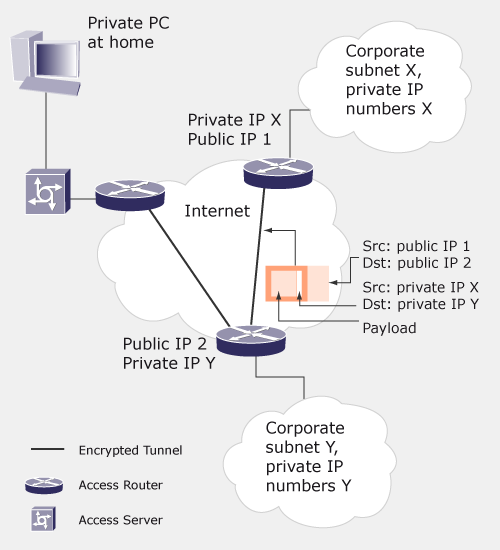
\includegraphics[width=0.50\textwidth]{figure_2_1.png}
		\caption{vpn-types and tunneling}
\end{figure}
\subsection{Subnet-to-Subnet VPN}
Verbindet geographisch getrennte private IP-Subnetzwerke. Der gesamte Datenverkehr, der von einem Subnetzwerk ausgeht und f�r das andere bestimmt ist, wird durch das �ffentliche "`getunnelt."'
\subsection{Access VPN}
 Erm�glicht Roaming-Usern den Zugriff auf das virtuelle Netzwerk von Home-Computern oder �ber einen beliebigen Internet-POP (Point of Presence). Auch hier wird das Tunneling benutzt; entweder �bernimmt ein Home-Computer die Rolle eine Tunnel-Endpunktes, oder der POP eines Internet Service Providers (ISP).
\section{Encapsulation}

\subsection{Link Layer VPNs (Layer 2)}
Beispiele f�r VPNS auf dieser Ebene sind Integrated Services Digital Network (ISDN), Frame Realy und Asynchronous Transfer Mode. Auch Virtual Local Networks funktionieren auf �hnliche Weise auf dieser Ebene.

\paragraph{Vorteile}
\begin{itemize}
\item Verbindungsorientiert, Pakete m�ssen nicht geroutet werden sondern werden �ber einmal erstellten Link �bertragen.
\item QoS auf dieser Ebene schon garantiert, muss nicht noch zus�tzlich implementiert werden.
\end{itemize}

\paragraph{Nachteile}
\begin{itemize}
\item Braucht homogene Netzwerkstruktur
\item IP-Ebene muss trotzdem noch verwaltet werden, Mehraufwand auf zwei Ebenen!
\end{itemize}

\subsection{Network Layer VPNs (Layer 3)}
IP Pakete werden als Payload in ein anderes IP Paket verpackt(IP in IP, {\em IPIP}), dann versendet. Dass innere Paket kann dabei verschl�sselt werden und garantiert so Sicherheit, das �ussere jedoch nicht. Der VPN Server dient dann als Interface, der den �usseren Header entfernt \& das innere Paket entschl�sselt. 

Firewalls k�nnen eingesetzt werden um verschl�sselte Verbindungen zu erzwingen. 
\newpage
\section{Security and the Internet Protocol}
Es gibt viele verschiedene Technologien, um die Kommunikation �ber das Internet sicherer zu machen. Viele davon sind aber an eine bestimmte Anwendung gekoppelt (in diesem Fall werden die Sicherheitsmechanismen auf dem Application Layer bereitgestellt).
\paragraph{Beispiele}
\begin{itemize}
	\item PGP ("`Pretty Good Privacy"') f�r die Verschl�sselung von E-Mails und Browser-basierte Authentifizierung
	\item SSL ("`Secure Sockets Layer"') f�r die Verschl�sselung des Datenverkehrt zwischen Web-Browser und Web-Server.
\end{itemize}
Nat�rlich ist das f�r grosse Firmen oder f�r einen ISP (Internet Service Provider) nicht geeignet, da morgen andere Applikationen �ber die heutigen Netzwerke laufen k�nnten.
\subsection{Possible Threats in the Internet}
VPNs m�ssen mindestens die folgenden drei Anforderungen erf�llen:
\begin{itemize}
	\item Authentication (Die Person, mit der man kommuniziert, ist die, f�r die sie sich ausgibt)
	\item Confidentiality \& Privacy (Niemand soll den Datenverkehrt belauschen k�nnen)
	\item Integrity (Daten d�rfen w�hrend der �bertragung nicht ver�ndert werden k�nnen)
\end{itemize}
\subsubsection{Spoofing}
Beim Spoofing gibt sich ein Angreifer als jemand anderes aus, indem er Pakete mit einer entsprechenden IP-Source-Adresse statt der eigenen versieht. Es ist eine allgemeine Tatsache, dass eine IP-Source-Adresse nicht vertrauensw�rdig ist.

\begin{figure}[!htb]
	\centering
	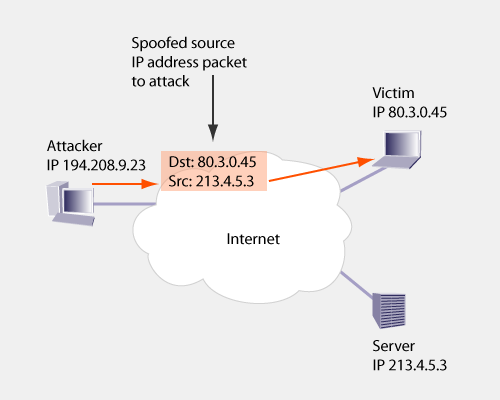
\includegraphics[width=0.50\textwidth]{figure_2_3.png}
\end{figure}
\subsubsection{Session Hijacking / Man in the Middle Attack}
Ein Hacker kann sich "`in die Mitte eines Kommunikationsweges setzen,"' und die Kommunikationspartner jeweils glauben lassen, er sei das Gegen�ber. Er kann s�mtliche Datenpakete filtern und manipulieren. Es reicht daher nicht aus, einen Kommunikations-partner \textit{einmal} zu identifizieren, sondern es sollte jede Datenquelle authentifiziert werden.
\begin{figure}[!htb]
	\centering
	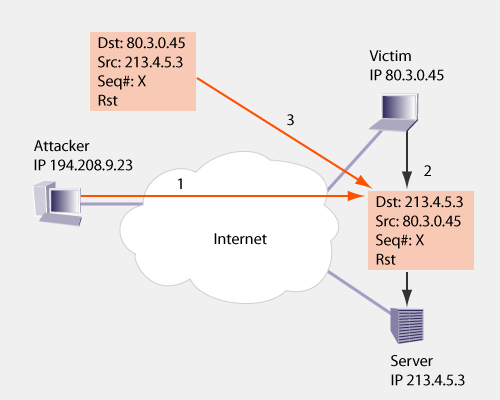
\includegraphics[width=0.50\textwidth]{figure_2_4.png}
\end{figure}
\subsubsection{Electronic Eavesdropping}
Ein grosser Teil der meisten Netzwerke basiert auf Ethernet LANs. Das Abh�ren solcher Ethernet-Leitungen ist einfach - noch ernster ist die Lage bei Wireless-LANs.
In Ethernet-Netzwerken kann jeder angeschlossene Knoten jedes Paket lesen. Es ist eine Konvention, dass jeder Knoten nur die an ihn adressierten Pakete verarbeitet. Nat�rlich kann ein Ger�t einfach konfiguriert werden, dass es alle Pakete "`sammmelt,"' �ber die Leitung verschickt werden. Physikalisch ist es nicht m�glich, an einem anderen Standort im Netzwerk festzustellen, dass ein Ger�t alle Pakete verarbeitet.
\newpage
\section[IP Sec]{IP Sec: The Security Architecture for the Internet Protocol}
Die IP Security Architecture (IPSec) bietet Sicherheits-Features f�r einzelne Datenpakete. Urspr�nglich wurde diese Architektur zur Verwendung in IPv6 konstruiert. Die IPSec-Architektur wurde aber auch in die bisherige IP-Version (IPv4) aufgenommen. IPSec enth�lt alle Sicherheitsmechanismen, die zur Implementierung von VPNs n�tig sind. \newline
Die IPSec-Architektur besteht aus verschiedenen Protokollen, die IP-Header-Erweiterungen beschreiben, die Sicherheitsmechanismen bereitstellen. Die Sicherheitsfunktionen f�r die einzelnen Pakete werden durch zwei Protokolle bereitgestellt:
\paragraph{AH}
Der Authentication Header stellt Datenintegrit�t und Authentizit�t sicher.
\paragraph{ESP}
Das Encapsulating Security Payload-Protokoll sorgt f�r Privacy mit Hilfe von Verschl�sselungsmechanismen.
\newline
\newline
AH und ESP sind unabh�ngige Protokolle, sie separat oder miteinander kombiniert eingesetzt werden k�nnen.
\subsection[ESP]{The Encapsulation Security Payload}
Das ESP hat die Protokollnummer 50. Die Nutzdaten werden umfasst von einem ESP-Header und einem ESP-Trailer.
\begin{figure}[!htb]
	\centering
		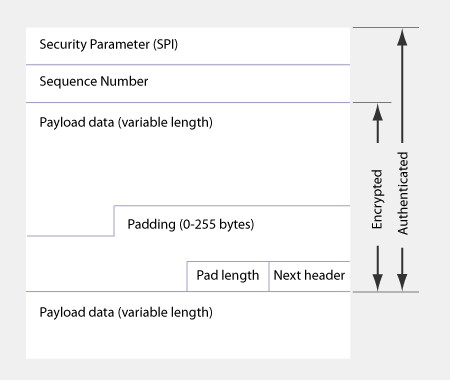
\includegraphics[width=0.50\textwidth]{figure_3_4.png}
\end{figure}
\newpage
\subsubsection{ESP header}
Der ESP-Header befindet sich zwischen IP- und TCP-/UDP-/...-Header. Er enth�lt einen sogenannten SPI (security parameter index), um die Sicherheits-Assoziation zu identifizieren, und eine Sequenznummer, die f�r jedes Datenpaket inkrementiert wird (Abwehr von Replay-Attacken).
\subsubsection{ESP trailer}
Der ESP-Trailer befindet sich hinter den Nutzdaten und ist, wie die Nutzdaten selbst, verschl�sselt. Der Trailer sorgt auch f�r das Padding (Auff�llen der Datenbl�cke), das n�tig ist, weil Verschl�sselungs-Algorithmen oft Datenbl�cke von einer bestimmten L�nge voraussetzen. Der Trailer enth�lt daher ein Feld, das die L�nge des Paddings in Bits enth�lt (pad length field). Ein weiteres Feld des ESP-Trailers enth�lt die Protokoll-Nummer des n�chsten Protokolls (z.B. IP oder ein ein n�chstes IPSec-Protokoll)
\subsection[AH]{The Authentication Header}
Das AH-Protokoll hat die Nummer 51. Es dient dazu, ein Datenpaket zu authentifizieren, so dass das IPSec-Peer des Empf�ngers sicher sein kann, von wo das erhaltene Paket stammt. Auch die Datenintegrit�t ist gew�hrleistet, d.h. die Empf�nger-Station kann �berpr�fen, dass kein Dritter das Paket w�hrend der �bertragung manipuliert hat. AH macht das durch das Berechnen von entsprechenden Authentifizierungs-Daten mit einer sicheren one-way Hash-Funktion. Da diese Berechnung mit Hilfe eines geheimen Schl�ssels geschieht. Ein Angreifer, der den geheimen Schl�ssel nicht kennt, ist nicht in der Lage, ein valides Datenpaket herauszufiltern oder zu authentifizieren. \newline Der AH-Header enth�lt ein Feld f�r den n�chsten Header und codiert die L�nge der Nutzdaten (n�tig, da die Authentifizierungsdaten variabel sind in ihrer L�nge). Wie der ESP-Header enth�lt auch der AH-Header einen SPI (Security Parameter Index) und eine Sequenznummer. Dahinter folgen dann die Authentifizierungsdaten (= der Wert der berechneten Hash-Funktion).
\begin{figure}[!htb]
	\centering
		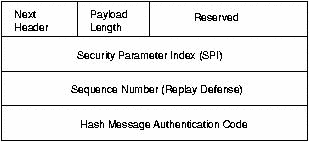
\includegraphics[width=0.50\textwidth]{ah_header.png}
\end{figure}

\section{Transport and Tunnel Mode}
... To do


\end{document}
